% !TeX program = xelatex
\documentclass[a4paper,10pt]{article}

% ============================================================================
% កញ្ចប់បណ្ណាល័យ (Packages) – តាមលំនាំស្តង់ដារ អនុវិទ្យាល័យព្រះក្រសាំង (ls_plan.tex)
% បរិបទ៖ ថ្នាក់រៀនគ្មានស្លាយ LCD – បង្រៀនដោយប្រើក្ដារខៀន សៀវភៅគោល និងសន្លឹកកិច្ចការស-ខ្មៅ
% ============================================================================
\usepackage[a4paper, left=0.95cm, right=0.95cm, top=0.85cm, bottom=0.92cm, footskip=0.52cm]{geometry}
\usepackage{amsmath}
\usepackage{unicode-math}
\usepackage{fontspec}
\usepackage{array, longtable, multirow, colortbl}
\usepackage[table]{xcolor}
\usepackage{enumitem}
\usepackage{pifont}
\usepackage{fancyhdr}
\usepackage{tikz}
\usetikzlibrary{calc, arrows.meta, positioning, babel}

\makeatletter
\let\@expl@@@mark@update@singlecol@structures@@\relax
\makeatother

\providecommand{\NGSFindFonts}{%
  \IfFileExists{C:/Windows/Fonts/cambria.ttc}{%
    \def\NGSSysPath{C:/Windows/Fonts/}%
    \def\NGSUserPath{C:/Users/KIT/AppData/Local/Microsoft/Windows/Fonts/}%
  }{%
    \IfFileExists{./fonts/KhmerOSsiemreap.ttf}{\def\NGSSysPath{./fonts/}\def\NGSUserPath{./fonts/}}{%
    \IfFileExists{../fonts/KhmerOSsiemreap.ttf}{\def\NGSSysPath{../fonts/}\def\NGSUserPath{../fonts/}}{%
    \IfFileExists{../../fonts/KhmerOSsiemreap.ttf}{\def\NGSSysPath{../../fonts/}\def\NGSUserPath{../../fonts/}}{%
    \IfFileExists{../../../fonts/KhmerOSsiemreap.ttf}{\def\NGSSysPath{../../../fonts/}\def\NGSUserPath{../../../fonts/}}{%
    \IfFileExists{../../../../fonts/KhmerOSsiemreap.ttf}{\def\NGSSysPath{../../../../fonts/}\def\NGSUserPath{../../../../fonts/}}{%
    \IfFileExists{../../../../../fonts/KhmerOSsiemreap.ttf}{\def\NGSSysPath{../../../../../fonts/}\def\NGSUserPath{../../../../../fonts/}}{%
    \IfFileExists{../../../../../../fonts/KhmerOSsiemreap.ttf}{\def\NGSSysPath{../../../../../../fonts/}\def\NGSUserPath{../../../../../../fonts/}}{%
      \def\NGSSysPath{../../../../../../../fonts/}\def\NGSUserPath{../../../../../../../fonts/}%
    }}}}}}}%
  }%
}
\NGSFindFonts

\setmathfont[Path={\NGSSysPath}, FontIndex=1, Scale=1.02]{cambria.ttc}
\defaultfontfeatures{Ligatures=TeX}

\setmainfont[
  Path={\NGSUserPath},
  Extension=.ttf,
  Script=Khmer,
  BoldFont={KhmerOSsiemreap},
  BoldFeatures={FakeBold=1.8},
  ItalicFont={KhmerOSsiemreap},
  ItalicFeatures={FakeSlant=0.25},
  BoldItalicFont={KhmerOSsiemreap},
  BoldItalicFeatures={FakeBold=1.8, FakeSlant=0.25}
]{KhmerOSsiemreap}

\newfontfamily\muol[Path={\NGSUserPath}, Extension=.ttf, Script=Khmer]{KhmerOSmuollight}
\newfontfamily\TimesEn[Path={\NGSSysPath}, Extension=.ttf, BoldFont={timesbd}, ItalicFont={timesi}, BoldItalicFont={timesbi}]{times}
\newfontfamily\NagaBold[Path={\NGSUserPath}, Extension=.ttf]{AKbalthom Naga Bold}
\newfontfamily\CalibriFont[Path={\NGSSysPath}, Extension=.ttf]{calibri}
\newfontfamily\Tacteing[Path={\NGSUserPath}]{TACTENG.TTF}
\newfontfamily\CourierBullet[Path={\NGSSysPath}, Extension=.ttf]{cour}
\newcommand{\wcirc}{{\CourierBullet\fontsize{9.5pt}{11pt}\selectfont o}}

\XeTeXlinebreaklocale "km"
\XeTeXlinebreakskip = 0pt plus 1pt minus 0.1pt

\definecolor{stepgray}{HTML}{D9D9D9}
\definecolor{headgray}{HTML}{F2F2F2}
\definecolor{boxgray}{HTML}{D9D9D9}
\definecolor{darkred}{HTML}{C00000}
\definecolor{red5e}{HTML}{FF0000}

\pagestyle{fancy}
\fancyhf{}
\renewcommand{\headrulewidth}{0pt}
\fancyfoot[R]{\CalibriFont\fontsize{11pt}{13pt}\selectfont\thepage}

\setlength{\parindent}{0pt}
\setlength{\parskip}{0pt}
\setlength{\tabcolsep}{3.8pt}

\newcolumntype{L}[1]{>{\raggedright\arraybackslash}p{#1}}

\newcommand{\en}[1]{{\TimesEn #1}}
\newcommand{\enbf}[1]{{\TimesEn\textbf{#1}}}
\newcommand{\unit}[1]{\,\text{\en{#1}}}
\newcommand{\fiveE}[1]{{\NagaBold\fontsize{9.5pt}{13pt}\selectfont\textcolor{red5e}{#1}}}
\newcommand{\timenote}[1]{\textcolor{darkred}{\textit{#1}}}
\newcommand{\graybox}[1]{\colorbox{boxgray}{\strut\hspace{2pt}#1\hspace{2pt}}}
\newcommand{\ditem}{\tikz[baseline=-0.5ex]\fill (0,0.42ex) -- (0.42ex,0) -- (0,-0.42ex) -- (-0.42ex,0) -- cycle;\hspace{0.3em}}
\newcommand{\cnum}[1]{{\fontsize{10.5pt}{12pt}\selectfont\ding{\numexpr171+#1\relax}}\hspace{0.2em}}
\newcommand{\cfig}[1]{\par\vspace{4pt}{\centering #1\par}\vspace{4pt}}
\newcommand{\stepheader}[1]{\multicolumn{3}{|c|}{\cellcolor{stepgray}\muol #1} \\* \noalign{\hrule height 0.4pt}}
\newcommand{\khmflourish}{{\Tacteing\fontsize{36pt}{14pt}\selectfont\raisebox{-5pt}{3}}}

% ============================================================================
% ម៉ាក្រូរូបភាពគរុកោសល្យស-ខ្មៅ (Proportional B&W TikZ Diagrams)
% ============================================================================

% ១. E1 Engage: ការេជ្រុង (a+b) បំបែកជា ៤ បំណែក (ទំ.៦៣) vs អន្ទាក់ (a+b)^2 = a^2 + b^2
\newcommand{\figEngageALGFive}{%
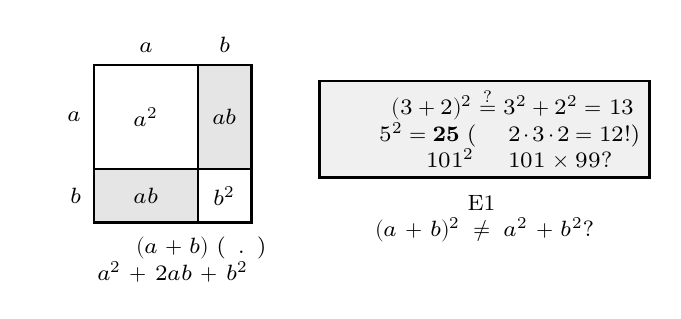
\begin{tikzpicture}[scale=0.80, every node/.style={font=\footnotesize, text=black}]
  % ឆ្វេង៖ ការេជ្រុង (a+b) (ទំ.៦៣)
  \begin{scope}[shift={(0,0)}]
    \draw[black, line width=1.0pt, fill=white] (0,0.85) rectangle (1.65,2.50);
    \draw[black, line width=1.0pt, fill=gray!20] (1.65,0.85) rectangle (2.50,2.50);
    \draw[black, line width=1.0pt, fill=gray!20] (0,0) rectangle (1.65,0.85);
    \draw[black, line width=1.0pt, fill=white] (1.65,0) rectangle (2.50,0.85);
    \node at (0.825,1.675) {$a^2$};
    \node at (2.075,1.675) {$ab$};
    \node at (0.825,0.425) {$ab$};
    \node at (2.075,0.425) {$b^2$};
    \node[above=1pt] at (0.825,2.50) {$a$};
    \node[above=1pt] at (2.075,2.50) {$b$};
    \node[left=1pt] at (0,1.675) {$a$};
    \node[left=1pt] at (0,0.425) {$b$};
    \node[anchor=north, text width=3.45cm, align=center] at (1.25,-0.08) {ការេជ្រុង $(a+b)$ (ទំ.៦៣)៖\\$a^2 + 2ab + b^2$};
  \end{scope}

  % ស្ដាំ៖ អន្ទាក់បាត់តួ 2ab និងល្បឿនគិតមាត់
  \begin{scope}[shift={(3.95,0)}]
    \node[draw=black, line width=0.9pt, fill=gray!12, text width=3.95cm, align=center, inner sep=3.5pt] (trapbox) at (2.25,1.48) {
      អន្ទាក់៖ $(3+2)^2 \stackrel{?}{=} 3^2 + 2^2 = 13$\\
      ការពិត៖ $5^2 = \mathbf{25}$ (ខ្វះ $2\cdot 3\cdot 2 = 12$!)\\
      ចុះគិតមាត់ $101^2$ និង $101\times 99$?
    };
    \node[below=2.5pt of trapbox, text width=4.05cm, align=center] {បេសកកម្ម E1៖ ហេតុអ្វី $(a+b)^2 \ne a^2+b^2$?};
  \end{scope}
\end{tikzpicture}}

% ២. E4 Elaborate: រូបធរណីមាត្រប្រៀបធៀប (a-b)^2 (ទំ.៦៤) និង a^2 - b^2 = (a-b)(a+b) (ទំ.៦៥)
\newcommand{\figDissectALGFive}{%
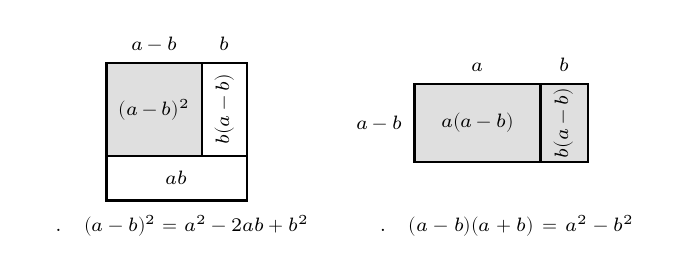
\begin{tikzpicture}[scale=0.76, every node/.style={font=\scriptsize, text=black}]
  % ឆ្វេង៖ (a-b)^2 (ទំ.៦៤)
  \begin{scope}[shift={(0,0)}]
    \draw[black, line width=0.95pt, fill=gray!25] (0,0.75) rectangle (1.60,2.30);
    \draw[black, line width=0.95pt, fill=white] (1.60,0.75) rectangle (2.35,2.30);
    \draw[black, line width=0.95pt, fill=white] (0,0) rectangle (2.35,0.75);
    \node at (0.80,1.525) {$(a-b)^2$};
    \node[rotate=90] at (1.975,1.525) {$b(a-b)$};
    \node at (1.175,0.375) {$ab$};
    \node[above=1pt] at (0.80,2.30) {$a-b$};
    \node[above=1pt] at (1.975,2.30) {$b$};
    \node[anchor=north, text width=3.55cm, align=center] at (1.175,-0.08) {ទំ.៦៤៖ $(a-b)^2 = a^2 - 2ab + b^2$};
  \end{scope}

  % ស្ដាំ៖ a^2 - b^2 = (a-b)(a+b) (ទំ.៦៥)
  \begin{scope}[shift={(5.15,0)}]
    \draw[black, line width=0.95pt, fill=gray!25] (0,0.65) rectangle (2.10,1.95);
    \draw[black, line width=0.95pt, fill=gray!25] (2.10,0.65) rectangle (2.90,1.95);
    \node at (1.05,1.30) {$a(a-b)$};
    \node[rotate=90] at (2.50,1.30) {$b(a-b)$};
    \node[left=1pt] at (0,1.30) {$a-b$};
    \node[above=1pt] at (1.05,1.95) {$a$};
    \node[above=1pt] at (2.50,1.95) {$b$};
    \node[anchor=north, text width=3.85cm, align=center] at (1.45,-0.08) {ទំ.៦៥៖ $(a-b)(a+b) = a^2 - b^2$};
  \end{scope}
\end{tikzpicture}}

\begin{document}
\fontsize{10pt}{15.2pt}\selectfont

% -------------------- ក្បាលកិច្ចតែងការ (Header) --------------------
\begin{center}
  {\muol\fontsize{11pt}{16pt}\selectfont ព្រះរាជាណាចក្រកម្ពុជា}\\[2pt]
  {\muol\fontsize{10pt}{15pt}\selectfont ជាតិ សាសនា ព្រះមហាក្សត្រ}\\[1pt]
  \khmflourish
\end{center}

\vspace{-28pt}
{\muol\fontsize{9.5pt}{12.5pt}\selectfont
មន្ទីរអប់រំ យុវជន និងកីឡា ខេត្តកំពង់ធំ\\
ការិយាល័យអប់រំ យុវជន និងកីឡា ស្រុកកំពង់ស្វាយ\\
អនុវិទ្យាល័យព្រះក្រសាំង}

\vspace{1pt}
\begin{center}
  {\muol\fontsize{10pt}{14pt}\selectfont កិច្ចតែងការបង្រៀន}
\end{center}
\vspace{0pt}

% -------------------- ព័ត៌មានទូទៅ (Metadata) --------------------
{\renewcommand{\arraystretch}{0.95}
\hspace*{4.05cm}%
\begin{tabular}{@{}l l l@{}}
  - \hspace{0.35cm} មុខវិជ្ជា & : & គណិតវិទ្យា ថ្នាក់ទី៨ \\
  - \hspace{0.35cm} ចំណងជើងមេរៀន & : & មេរៀនទី៥ កន្សោមពីជគណិត \\
  - \hspace{0.35cm} ចំណងជើងរង & : & ៣.១ សមភាពសំខាន់ៗ៖ ពន្លាតការេនៃទ្វេធា និងផលគុណទ្វេធាឆ្លាស់សញ្ញា \\
  - \hspace{0.35cm} រយៈពេល & : & ១ ម៉ោងសិក្សា (៥០ នាទី) \\
  - \hspace{0.35cm} បង្រៀនដោយ & : & ហុក ប៊ុនថែន \\
  - \hspace{0.35cm} កាលបរិច្ឆេទ & : & ថ្ងៃពុធ ១៥រោច ខែកត្តិក ព.ស.២៥៧០ (៩ ធ្នូ ២០២៦) \\
\end{tabular}
}

\vspace{1pt}

% -------------------- I. វត្ថុបំណង --------------------
\textbf{I.} {\muol វត្ថុបំណង}\\[1pt]
\hspace*{0.55cm}%
\begin{tabular}{@{}l l L{14.2cm}@{}}
  \wcirc \hspace{0.25cm} វិជ្ជាសម្បទា & : & សិស្សប្រាប់បានត្រឹមត្រូវនូវរូបមន្តសមភាពសំខាន់ៗទាំង ៣ គឺ \textbf{ការេនៃផលបូក} $(a+b)^2 = a^2+2ab+b^2$, \textbf{ការេនៃផលដក} $(a-b)^2 = a^2-2ab+b^2$ និង \textbf{ផលគុណទ្វេធាឆ្លាស់សញ្ញា} $(a-b)(a+b) = a^2-b^2$ តាមសៀវភៅគោល ទំ.៦៣--៦៦ ។ \\
  \wcirc \hspace{0.25cm} បំណិនសម្បទា & : & សិស្សបកស្រាយសមភាពទាំង ៣ តាមផ្ទៃក្រឡាធរណីមាត្រ និងតាមពិជគណិត ព្រមទាំងអនុវត្តពន្លាតកន្សោមពីជគណិត និងគិតលេខមាត់រហ័ស ($101^2, 99^2, 101\times 99$) បានត្រឹមត្រូវ ។ \\
  \wcirc \hspace{0.25cm} ចរិយាសម្បទា & : & សិស្សមានភាពប្រុងប្រយ័ត្នមិនភ្លេចតួកណ្ដាល $\pm 2ab$ ក្នុងការេនៃទ្វេធា និងចូលចិត្តប្រើសមភាពសំខាន់ៗដើម្បីគិតលេខរហ័សក្នុងជីវភាព ។ \\
\end{tabular}

\vspace{1pt}

% -------------------- II. សម្ភារៈឧបទេស --------------------
\textbf{II.} {\muol សម្ភារៈឧបទេស}\\[1pt]
\hspace*{0.55cm}$\bullet$ \hspace{0.35cm} សៀវភៅសិក្សាគោលគណិតវិទ្យាថ្នាក់ទី៨ (ទំ.៦៣--៦៦ និងទំ.៧៣) ក្ដារខៀន ដីស បន្ទាត់ និងសន្លឹកកិច្ចការសិស្សស-ខ្មៅ (\en{Worksheet\_ALG55} ចំនួន ២ ទំព័រ \en{A4} ដោយគ្មានស្លាយ \en{LCD}) ។

\vspace{1pt}

% -------------------- III. វិធីសាស្រ្តបង្រៀន --------------------
\textbf{III.} {\muol វិធីសាស្រ្តបង្រៀន}\\[1pt]
\hspace*{0.55cm}$\bullet$ \hspace{0.35cm} គោលវិធីសិស្សមជ្ឈមណ្ឌលតាមគំរូ \en{5Es} រួមបញ្ចូល \textbf{ការបំបែកផ្ទៃក្រឡាធរណីមាត្រ និងការបដិសេធអន្ទាក់បាត់តួកណ្ដាល $2ab$} (\en{Geometric Area-Dissection \& Freshman's-Dream Refutation}; \en{Fitria et al., 2023; Aydin-G\"u\c{c} \& Ayg\"un, 2021}) ។

\vspace{2pt}

% -------------------- IV. ដំណើរការបង្រៀន --------------------
\textbf{IV.} {\muol ដំណើរការបង្រៀន}\\[-6pt]

{\renewcommand{\arraystretch}{1.15}
\begin{longtable}{|L{5.50cm}|L{7.90cm}|L{4.80cm}|}
\hline
\multicolumn{1}{|c|}{\cellcolor{headgray}\muol សកម្មភាពគ្រូ} &
\multicolumn{1}{c|}{\cellcolor{headgray}\muol ខ្លឹមសារមេរៀន} &
\multicolumn{1}{c|}{\cellcolor{headgray}\muol សកម្មភាពសិស្ស} \\[2pt]
\hline
\endfirsthead

\hline
\multicolumn{1}{|c|}{\cellcolor{headgray}\muol សកម្មភាពគ្រូ} &
\multicolumn{1}{c|}{\cellcolor{headgray}\muol ខ្លឹមសារមេរៀន} &
\multicolumn{1}{c|}{\cellcolor{headgray}\muol សកម្មភាពសិស្ស} \\[2pt]
\hline
\endhead

\hline
\endfoot

% ==================== ជំហានទី១ (2min) ====================
\stepheader{ជំហានទី១ ៖ រដ្ឋបាលថ្នាក់ (២ នាទី)}
$\bullet$ ពិនិត្យអវត្តមាន សណ្ដាប់ធ្នាប់ អនាម័យ និងសៀវភៅគោល \par\vspace{1pt}
$\bullet$ ចែកសន្លឹកកិច្ចការស-ខ្មៅ \en{Worksheet\_ALG55} ដល់សិស្សគ្រប់គ្នា
&
$\bullet$ វត្តមានសិស្ស ឯកសណ្ឋាន និងសណ្ដាប់ធ្នាប់ថ្នាក់រៀន \par
$\bullet$ សន្លឹកកិច្ចការសិស្ស \en{Worksheet\_ALG55} (ទំព័រ ១--២) លើតុរៀងៗខ្លួន
&
$\circ$ ប្រធានថ្នាក់រាយការណ៍អវត្តមាន \par
$\circ$ សរសេរឈ្មោះលើសន្លឹកកិច្ចការ \\
\hline

% ==================== ជំហានទី២ (9min) ====================
\stepheader{ជំហានទី២ ៖ កែកិច្ចការផ្ទះ រំលឹកមេរៀនចាស់ និងភ្ជាប់បញ្ហាថ្មី (៩ នាទី)}
\ditem \textbf{កែកិច្ចការផ្ទះ ($\le 3\unit{min}$)៖} \par
$\bullet$ ហៅសិស្ស ១ រូបឡើងកែលំហាត់ ៣គ (ទំ.៧២) និងលំហាត់ ៦ (ទំ.៧៣) លើក្ដារខៀន
&
\textbf{កំណែកិច្ចការផ្ទះ (សៀវភៅគោល ទំ.៧២--៧៣)៖} \par
១) $(x^2+2y)(x+1) = \mathbf{x^3 + x^2 + 2xy + 2y}$ ។ \par
២) $a(x-b) - b(a-x) + x(a+b) = ax - ab - ab + bx + ax + bx = \mathbf{2(a+b)x - 2ab}$ ។
&
$\circ$ ផ្ទៀងផ្ទាត់សញ្ញា $-b(-x) = +bx$ និងកែចម្លើយក្នុងសៀវភៅ \\[3pt]

\ditem \textbf{រំលឹកមេរៀនចាស់ ($3\unit{min}$)៖} \par
$\bullet$ សួររំលឹកពីការលើកឯកធាជាការេ និងការគុណទ្វេធា $(x+3)(x+3)$
&
\textbf{សំណួររំលឹកមូលដ្ឋានគ្រឹះ៖} \par
១) គណនា៖ $(2m)^2 = \mathbf{4m^2}$ \quad;\quad $\left(\frac{1}{2}m\right)^2 = \mathbf{\frac{1}{4}m^2}$ ។ \par
២) គុណទ្វេធា៖ $(x+3)(x+3) = x^2 + 3x + 3x + 9 = \mathbf{x^2 + 6x + 9}$ ។
&
$\circ$ ឆ្លើយផ្ទាល់មាត់ពីការលើកមេគុណជាការេ និងការបង្រួម $3x+3x=6x$ \\[3pt]

\fiveE{E1 - Engage} \timenote{(3 នាទី)} \par\vspace{1pt}
$\bullet$ គូសការេជ្រុង $(a+b)$ (ទំ.៦៣) លើក្ដារខៀន និងដាក់បញ្ហាអន្ទាក់ $(3+2)^2 \stackrel{?}{=} 3^2+2^2$ រួមនឹងល្បឿនគិតមាត់ $101^2$
&
\textbf{ស្ថានភាពភ្ជាប់បញ្ហា៖ អន្ទាក់បាត់តួកណ្ដាល និងល្បិចគិតមាត់ $5$ វិនាទី!} \par
សិស្សម្នាក់ពន្លាត $(a+b)^2 = a^2 + b^2$ ។ បើជំនួស $a=3, b=2$ គេបាន $(3+2)^2 = 5^2 = \mathbf{25}$ ខណៈ $3^2+2^2 = 9+4 = \mathbf{13}$ (ខុសគ្នាដល់ទៅ $12$)! \par
\hspace*{0.3em}– \textbf{សំណួរបេសកកម្ម៖} «តើផ្ទៃក្រឡាប្រអប់ណាខ្លះដែលបាត់? ហើយធ្វើដូចម្ដេចគិតមាត់ $101^2$ និង $101\times 99$ បានភ្លាមៗ?»
&
$\circ$ ពិនិត្យភាពខុសគ្នារវាង $25$ និង $13$ \par
$\circ$ គូសធីកការទស្សន៍ទាយមុនរៀនក្នុងផ្នែកទី១ នៃសន្លឹកកិច្ចការ \\[3pt]

& \cfig{\figEngageALGFive} & \\
\hline

% ==================== ជំហានទី៣ (17min) ====================
\stepheader{ជំហានទី៣ ៖ មេរៀនថ្មី — ពន្លាតការេនៃទ្វេធា និងផលគុណទ្វេធាឆ្លាស់សញ្ញា (១៧ នាទី)}
\fiveE{E2 - Explore} \timenote{(11 នាទី)} \par\vspace{1pt}
\ditem \textbf{សកម្មភាពទី១៖ រុករកការេនៃផលបូក និងការេនៃផលដក ($5.5\unit{min}$)៖} \par
$\bullet$ ឱ្យសិស្សធ្វើការជាដៃគូលើ \textbf{ផ្នែកទី២ (ក)} នៃ \en{Worksheet\_ALG55} ដើម្បីទាញរូបមន្ត $(a+b)^2$ និង $(a-b)^2$ តាមផ្ទៃក្រឡា និងតាមពិជគណិត (ទំ.៦៣--៦៤)
&
\textbf{ការរុករកទី១ (ពន្លាត $(a+b)^2$ និង $(a-b)^2$ ទំ.៦៣--៦៤)៖} \par
$\bullet$ \textbf{ការេនៃផលបូក៖} $(a+b)(a+b) = a^2 + ab + ab + b^2 = \mathbf{a^2 + 2ab + b^2}$ \en{(1)} (មានតួកណ្ដាល $+2ab$ ជាផ្ទៃចតុកោណកែង $ab$ ពីរ!) ។ \par
$\bullet$ \textbf{ការេនៃផលដក៖} $(a-b)(a-b) = a^2 - ab - ab + (-b)^2 = \mathbf{a^2 - 2ab + b^2}$ \en{(2)} \textit{(ប្រយ័ត្ន៖ តួចុងក្រោយគឺ $\mathbf{+b^2}$ ជានិច្ច មិនមែន $-b^2$ ទេ!)} ។
&
$\circ$ បូកផ្ទៃក្រឡាបំណែកទាំង ៤ ក្នុងសន្លឹកកិច្ចការ \par
$\circ$ កត់សម្គាល់ថាតួចុងក្រោយនៃ $(a-b)^2$ គឺ $+b^2$ ព្រោះ $(-b)(-b)=+b^2$ \\[3pt]

\ditem \textbf{សកម្មភាពទី២៖ រុករកផលគុណទ្វេធាឆ្លាស់សញ្ញា ($5.5\unit{min}$)៖} \par
$\bullet$ ឱ្យដៃគូបន្តបំពេញ \textbf{ផ្នែកទី២ (ខ)}៖ គុណ $(a-b)(a+b)$ និងផ្ទៀងផ្ទាត់តាមរូបផ្ទៃក្រឡាផ្នែកប្រផេះ (ទំ.៦៥)
&
\textbf{ការរុករកទី២ (ពន្លាត $(a-b)(a+b)$ ទំ.៦៥)៖} \par
$\bullet$ តាមពិជគណិត៖ $(a-b)(a+b) = a^2 + ab - ab - b^2 = \mathbf{a^2 - b^2}$ \en{(3)} (តួកណ្ដាល $+ab$ និង $-ab$ ស៊ីសងគ្នាអស់សូន្យ!) ។ \par
$\bullet$ តាមធរណីមាត្រ (ទំ.៦៥)៖ ការេធំ $a^2$ ដកការេតូច $b^2$ បំបែកផ្គុំឡើងវិញបានចតុកោណកែងទទឹង $(a-b)$ និងបណ្ដោយ $(a+b)$ ។
&
$\circ$ ឃើញច្បាស់ថា $+ab - ab = 0$ ធ្វើឱ្យសល់តែ ២ តួគឺ $a^2 - b^2$ \\[3pt]

\fiveE{E3 - Explain} \timenote{(6 នាទី)} \par\vspace{1pt}
$\bullet$ ហៅតំណាងដៃគូឡើងសរសេរសមភាពទាំង ៣ រួចគ្រូសង្ខេបធនាគារហេតុផល \cnum{1}--\cnum{5} លើក្ដារខៀន
&
\textbf{សង្ខេបខ្លឹមសារគោល៖ ៣.១ សមភាពសំខាន់ៗទាំង ៣ (ទំ.៦៣--៦៥)} \par
$\bullet$ \cnum{1} \textbf{រូបមន្តទី១៖} $(a + b)^2 = a^2 + 2ab + b^2$ (មានសញ្ញា $+$ ដូចគ្នាត្រង់ $+2ab$) ។ \par
$\bullet$ \cnum{2} \textbf{រូបមន្តទី២៖} $(a - b)^2 = a^2 - 2ab + b^2$ (មានសញ្ញា $-$ ត្រង់ $-2ab$, តែ $+b^2$) ។ \par
$\bullet$ \cnum{3} \textbf{រូបមន្តទី៣៖} $(a - b)(a + b) = a^2 - b^2$ (ផលដកនៃពីរការេ) ។
&
$\circ$ ឡើងសរសេរ និងប្រៀបធៀបសញ្ញានៃសមភាពទាំង ៣ \\[3pt]

$\bullet$ បញ្ជាក់គន្លឹះលើកមេគុណជាការេ (\cnum{4}) និងគិតលេខមាត់ (\cnum{5})
&
$\bullet$ \cnum{4} \textbf{របាំងមេគុណ៖} ត្រូវដាក់វង់ក្រចកលើកទាំងមេគុណជាការេ ឧ. $(2m)^2 = 4m^2$ ។ \par
$\bullet$ \cnum{5} \textbf{គិតមាត់រហ័ស៖} បំបែកលេខជិត $100$ ជា $(100\pm k)^2$ ឬ $(100+k)(100-k)$ ។
&
$\circ$ កត់ត្រារូបមន្ត \cnum{1}--\cnum{5} ចូលក្នុងប្រអប់ផ្នែកទី៣ នៃសន្លឹកកិច្ចការ \\
\hline

% ==================== ជំហានទី៤ (20min) ====================
\stepheader{ជំហានទី៤ ៖ ពង្រីកចំណេះដឹង និងវាយតម្លៃលទ្ធផលសិក្សា (២០ នាទី)}
\fiveE{E4 - Elaborate} \timenote{(10 នាទី)} \par\vspace{1pt}
\ditem \textbf{លំហាត់គំរូពន្លាតកន្សោមពីជគណិត (ទំ.៦៣--៦៥, $5\unit{min}$)៖} \par
$\bullet$ ដឹកនាំសិស្សដោះស្រាយលំហាត់គំរូទី១ និងទី២ នៃរូបមន្តទាំង ៣ ក្នុង \textbf{ផ្នែកទី៤ (១)} នៃសន្លឹកកិច្ចការ
&
\textbf{លំហាត់គំរូពន្លាតកន្សោម (សៀវភៅគោល ទំ.៦៣--៦៥)៖} \par
$\bullet$ គំរូទី១៖ $(x+3)^2 = \mathbf{x^2 + 6x + 9}$ \;;\; $(x-1)^2 = \mathbf{x^2 - 2x + 1}$ \;;\; $(x-2)(x+2) = \mathbf{x^2 - 4}$ ។ \par
$\bullet$ ទំ.៦៣៖ $(2m + 3n)^2 = (2m)^2 + 2(2m)(3n) + (3n)^2 = \mathbf{4m^2 + 12mn + 9n^2}$ ។ \par
$\bullet$ ទំ.៦៤៖ $\left(\frac{1}{2}m - n\right)^2 = \left(\frac{1}{2}m\right)^2 - 2\left(\frac{1}{2}m\right)(n) + n^2 = \mathbf{\frac{1}{4}m^2 - mn + n^2}$ ។ \par
$\bullet$ ទំ.៦៥៖ $\left(\frac{1}{2}m - 3n\right)\left(\frac{1}{2}m + 3n\right) = \left(\frac{1}{2}m\right)^2 - (3n)^2 = \mathbf{\frac{1}{4}m^2 - 9n^2}$ ។
&
$\circ$ កំណត់តួ $A$ និង $B$ ច្បាស់ និងដាក់វង់ក្រចកលើកមេគុណជាការេលើសន្លឹកកិច្ចការ \\[3pt]

\ditem \textbf{គិតមាត់រហ័ស និងកំសាន្តគណិតវិទ្យា (ទំ.៦៣--៦៦, $5\unit{min}$)៖} \par
$\bullet$ ដឹកនាំសិស្សគណនា $101^2,\; 99^2,\; 101\times 99$ និងរកលំនាំ «កំសាន្តគណិតវិទ្យា» ទំ.៦៦
&
\textbf{លំហាត់គំរូទី៣ (គិតមាត់) និងកំសាន្តគណិតវិទ្យា (ទំ.៦៤--៦៦)៖} \par
$\bullet$ $101^2 = (100+1)^2 = 10000 + 200 + 1 = \mathbf{10201}$ \;;\; $99^2 = (100-1)^2 = 10000 - 200 + 1 = \mathbf{9801}$ \;;\; $101\times 99 = 100^2 - 1^2 = \mathbf{9999}$ ។ \par
$\bullet$ \textbf{កំសាន្តគណិតវិទ្យា (ទំ.៦៦)៖} $(1+1)(1-1)=0$, $(2+1)(2-1)=3$, $(3+2)(3-2)=5$, $(4+3)(4-3)=\mathbf{7}$, $\dots$, $(10+9)(10-9)=\mathbf{19}$ ។ \par
$\bullet$ \textbf{ឆ្លុះបញ្ចាំង៖} ចំពោះចំនួនគត់តគ្នា $n$ និង $n-1$ គេបាន $(n+(n-1))(n-(n-1)) = n^2 - (n-1)^2 = \mathbf{2n - 1}$ ។
&
$\circ$ គណនាលេខមាត់ និងបកស្រាយលំនាំផលដកការេនៃពីរចំនួនតគ្នា \\[3pt]

& \cfig{\figDissectALGFive} & \\[3pt]

\fiveE{E5 - Evaluate} \timenote{(10 នាទី)} \par\vspace{1pt}
\ditem \textbf{អនុវត្ត «ប្រតិបត្តិ» ទំ.៦៤ និងទំ.៦៥ ($6.5\unit{min}$)៖} \par
$\bullet$ ឱ្យសិស្សធ្វើលំហាត់ \textbf{ប្រតិបត្តិ} ទំ.៦៤ ដោយខ្លួនឯងក្នុងផ្នែកទី៥ (១) នៃសន្លឹកកិច្ចការ
&
\textbf{ចម្លើយលំហាត់ «ប្រតិបត្តិ» (សៀវភៅគោល ទំ.៦៤ និងទំ.៦៥)៖} \par
១) \textbf{ទំ.៦៤ $(a+b)^2$៖} ក) $(b+2a)^2 = \mathbf{b^2 + 4ab + 4a^2}$ \;;\; ខ) $(5x+2y)^2 = \mathbf{25x^2 + 20xy + 4y^2}$ \;;\; គ) $(6x^2+4)^2 = \mathbf{36x^4 + 48x^2 + 16}$ \;;\; ឃ) $(a+5)^2 = \mathbf{a^2 + 10a + 25}$ ។
&
$\circ$ ពន្លាត $(6x^2+4)^2$ ដោយប្រយ័ត្ន $(6x^2)^2 = 36x^4$ \\[3pt]

$\bullet$ ឱ្យសិស្សបន្តធ្វើ \textbf{ប្រតិបត្តិ} ទំ.៦៥ រួចប្ដូរសន្លឹកកិច្ចការផ្ទៀងជាដៃគូ
&
២) \textbf{ទំ.៦៥ $(a-b)^2$៖} ក) $(x-2y)^2 = \mathbf{x^2 - 4xy + 4y^2}$ \;;\; ខ) $(5b-y)^2 = \mathbf{25b^2 - 10by + y^2}$ \;;\; គ) $(x-4y)^2 = \mathbf{x^2 - 8xy + 16y^2}$ \;;\; ឃ) $\left(\frac{1}{5}a - 5\right)^2 = \mathbf{\frac{1}{25}a^2 - 2a + 25}$ ។
&
$\circ$ ប្ដូរសន្លឹកកិច្ចការផ្ទៀងផ្ទាត់តួកណ្ដាល $-2\cdot\frac{1}{5}a\cdot 5 = -2a$ (\en{Pause-Review}) \\[3pt]

\ditem \textbf{បិទបេសកកម្ម E1 និងតេស្តរហ័ស \en{Exit Check} ($3.5\unit{min}$)៖} \par
$\bullet$ សួរបិទបេសកកម្ម E1 និងឱ្យសិស្សគូសរង្វង់ជម្រើស \en{A--D}
&
$\bullet$ \textbf{បិទបេសកកម្ម E1៖} $(a+b)^2$ មានតួកណ្ដាល $\mathbf{+2ab}$ ហើយ $101^2 = 10201,\; 101\times 99 = 9999$ ។ \par
$\bullet$ \textbf{Exit Check៖} តើពន្លាតនៃ $(3x - 4y)^2$ ស្មើនឹងកន្សោមមួយណា? \par
\en{A.} $9x^2 - 16y^2$ \quad \en{B.} $9x^2 - 12xy + 16y^2$ \quad \graybox{\enbf{C.} $9x^2 - 24xy + 16y^2$ \ding{51}} \quad \en{D.} $9x^2 - 24xy - 16y^2$
&
$\circ$ គណនា $-2(3x)(4y) = -24xy$ និង $+16y^2$ រួចគូសរង្វង់ជម្រើស \textbf{C} \\
\hline

% ==================== ជំហានទី៥ (<=2min) ====================
\stepheader{ជំហានទី៥ ៖ កិច្ចការផ្ទះ និងបណ្ដាំផ្ញើ ($\le$ ២ នាទី)}
$\bullet$ កត់ត្រាកិច្ចការផ្ទះលើក្ដារខៀន (មានបោះពុម្ពស្រាប់នៅផ្នែកទី៦ នៃសន្លឹកកិច្ចការទំព័រទី២) \par
$\bullet$ ណែនាំគំរូ $39\times 41 = (40-1)(40+1)$ សម្រាប់លំហាត់ទី៩
&
\textbf{កិច្ចការផ្ទះ (សៀវភៅសិក្សាគោល ទំ.៧៣)៖} \par
១. \textbf{លំហាត់ទី៨ ក៖} ស្រាយបញ្ជាក់សមភាព $(1 + x)(1 - x)(1 + x^2) = 1 - x^4$ ។ \par
២. \textbf{លំហាត់ទី៩៖} មុធាគណនាដោយប្រើសមភាពសំខាន់ៗ៖ $39\times 41,\; 54\times 66,\; 19\times 21,\; 39^2,\; 102^2 - 101^2,\; 54^2 - 46^2$ ។ \par
៣. \textbf{លំហាត់ទី១០ គ និង ឃ៖} ពន្លាត និងបង្រួម៖ គ) $(a - 3b)^2 + 9(a^2 - 3b) + 5$ \;;\; ឃ) $-x(4x - 3y) + x^2 - 12xy$ ។
&
$\circ$ កត់ត្រាកិច្ចការផ្ទះ និងទុកដាក់សន្លឹកកិច្ចការក្នុងសឺមីគណិតវិទ្យា \\[3pt]

$\bullet$ ណែនាំឱ្យអានចំណុច ៣.២ ជាមុនសម្រាប់ម៉ោងក្រោយ
&
$\bullet$ \textbf{អានជាមុន៖} ចំណុច \textbf{៣.២ ពន្លាតគូបនៃទ្វេធា និងត្រីកោណប៉ាស្កាល់} (សៀវភៅគោល ទំព័រ ៦៦--៦៨) ។
&
$\circ$ ទទួលបណ្ដាំផ្ញើ និងជម្រាបលាគ្រូ \\

\end{longtable}
}

\vspace{6pt}

% -------------------- ហត្ថលេខា (Signature Block) --------------------
\begin{flushright}
\begin{minipage}{9.6cm}
\centering
ថ្ងៃពុធ ១៥រោច ខែកត្តិក ឆ្នាំមមី អដ្ឋស័ក ពុទ្ធសករាជ ២៥៧០\\[2pt]
ព្រះក្រសាំង, ថ្ងៃទី៩ ខែធ្នូ ឆ្នាំ២០២៦\\[4pt]
{\muol គ្រូបង្រៀន}\\[32pt]
\hfill{\muol ហុក ប៊ុនថែន}\hspace*{1.4cm}
\end{minipage}
\end{flushright}

\end{document}
